\begin{pa} \label{PA:10.3} Once again, let's consider the function $f$ defined by $ f(x,y) = \frac{x^2\sin(2y)}{32}$ 
  \begin{figure}[ht]
    \begin{center}
      \includegraphics{figures/fig_10_2_trace_x_a.eps}
      \hspace*{20pt}
      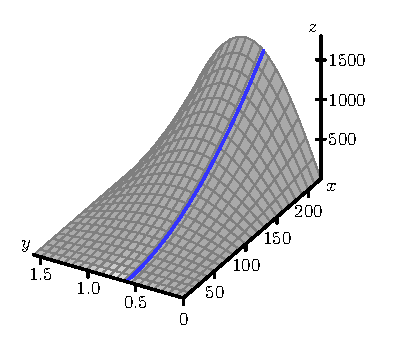
\includegraphics{figures/fig_10_2_trace_y_a.eps}
    \end{center}
    \caption{The range function with traces $y=0.6$ and $x=150$.}
    \label{F:10.3.preview}
  \end{figure}
that measures a projectile's range as a function of its
  initial speed $x$ and launch angle $y$.  The graph of this function,
  including traces with $x=150$ and $y=0.6$, is shown in Figure
  \ref{F:10.3.preview}. 

  \ba
  \item Compute the partial derivative $f_x$ and notice that $f_x$ itself is a
    new function of $x$ and $y$.
  \item We may now compute the partial derivatives of $f_x$.  Find the
    partial derivative $f_{xx} = (f_x)_x$ and evaluate $f_{xx}(150,
    0.6)$.  

  \item Figure \ref{F:10.3.preview.xx} shows the trace of $f$ with
    $y=0.6$ with three tangent lines included.  Explain how your
    result from part (b) of this preview activity is reflected in
    this figure.  

  \begin{figure}[ht]
    \begin{center}
      \scalebox{0.8}{\includegraphics{figures/fig_10_3_preview_xx.eps}}
    \end{center}
    \caption{The trace with $y=0.6$.}
    \label{F:10.3.preview.xx}
  \end{figure}

%\item Still considering $f_x$, compute its other partial derivative,
%  $f_{xy} = (f_x)_y$, and evaluate $f_{xy}(150, 0.6)$.
  
%  \item Figure \ref{F:10.3.preview.xy} shows the traces $f(x,b)$ with
 %   $b=0.4$, $b=0.6$, and $b=0.8$ with tangent lines at $x=150$
 %   included.  Explain how your 
 %   result from the previous part of this activity is reflected in
 %   this figure.  

%  \begin{figure}[ht]
%    \begin{center}
%      \scalebox{0.8}{\includegraphics{figures/fig_10_3_preview_yx.eps}}
%    \end{center}
%    \caption{The traces with $y=0.4$, $y=0.6$ and $y=0.8$.}
%    \label{F:10.3.preview.xy}
%  \end{figure}

  \item Determine the partial derivative $f_y$, and then find the partial
    derivative $f_{yy}=(f_y)_y$.  Evaluate $f_{yy}(150, 0.6)$.

%  \item The left side of Figure \ref{F:10.3.preview.y} shows traces
%    $f(a, y)$ with $a=125$, $a=150$, and $a=175$.  Explain how the
%    value of $f_{yx}(150,0.6)$ is reflected in this figure.  

  \begin{figure}[ht]
    \begin{center}
%      \includegraphics{figures/fig_10_3_preview_xy.eps}
%      \hspace*{20pt}
      \includegraphics{figures/fig_10_3_preview_yy.eps}
    \end{center}
    \caption{More traces of the range function.}
    \label{F:10.3.preview.y}
  \end{figure}

  \item Figure \ref{F:10.3.preview.y} shows the
    trace $f(150, y)$ and includes three tangent lines.
    Explain how the value of $f_{yy}(150,0.6)$ is reflected in this figure.  

%  \item What do you notice about the relationship between $f_{xy}$ and
%    $f_{yx}$?  

  \item Because $f_x$ and $f_y$ are each functions of both $x$ and $y$, they each have two partial derivatives.  Not only can we compute $f_{xx} = (f_x)_x$, but also $f_{xy} = (f_x)_y$; likewise, in addition to $f_{yy} = (f_y)_y$, but also $f_{yx} = (f_y)_x$.  For the range function $f(x,y) = \frac{x^2\sin(2y)}{32}$, use your earlier computations of $f_x$ and $f_y$ to now determine $f_{xy}$ and $f_{yx}$.  Write one sentence to explain how you calculated these ``mixed'' partial derivatives.

    \ea


\end{pa} 

\begin{activitySolution} 
  \ba
  \item The partial derivative $f_x$ is given by
    \[f_x(x,y) = \frac{2x\sin(2y)}{32} = \frac{x\sin(2y)}{16}.\]
 
  \item Differentiating $f_x$ with respect to $x$ yields
\[f_{xx}(x,y) = (f_x)_x(x,y) = \frac{\sin(2y)}{16}.\]
So $f_{xx}(150,0.6) = \frac{1}{16} \sin(1.2) \approx 0.058$. 

  \item The partial derivative $f_{xx} = (f_x)_x$ tells us how $f_x$ changes as we increase $x$ while $y$ remains constant. Now $f_x$ represents the slope of the tangent line to the trace of $f$ in the $x$ direction, so the fact that $f_{xx}(150,0.6) \approx 0.058$ tells us that the slopes of the tangent lines to the trace of $f$ in the $x$-direction are increasing by approximately 0.058 for every one unit increase in $x$ from $150$ if $y$ remains constant at $0.06$. This is reflected in the small increases in the slopes of the tangent lines as $x$ increases in the figure.  

  \item The partial derivative $f_y$ is given by
    \[f_y(x,y) = \frac{2x^2\cos(2y)}{32} = \frac{x^2\cos(2y)}{16}.\]
 Differentiating $f_y$ with respect to $y$ yields
\[f_{yy}(x,y) = (f_y)_y(x,y) = \frac{-2x^2\sin(2y)}{16} = -\frac{x^2\sin(2y)}{8}.\]
So $f_{yy}(150,0.6) = -\frac{150^2}{8} \sin(1.2) \approx -2621.36$. 


  \item The partial derivative $f_{yy} = (f_y)_y$ tells us how $f_y$ changes as we increase $y$ while $x$ remains constant. Now $f_y$ represents the slope of the tangent line to the trace of $f$ in the $y$ direction, so the fact that $f_{yy}(150,0.6) \approx -2621.36$ tells us that the slopes of the tangent lines to the trace of $f$ in the $y$-direction are decreasing by approximately 2621.26 for every one unit increase in $y$ from $0.6$ if $x$ remains constant at $150$. This is reflected in slopes in the figure decreasing from positive to negative. 

  \item If we treat $x$ as constant in $f_x$ and differentiate with respect to $y$ we obtain
\[f_{xy}(x,y) = (f_x)_y(x,y) = \frac{2x\cos(2y)}{16} = \frac{x\cos(2y)}{8}.\]
Similarly, if we treat $y$ as constant in $f_y$ and differentiate with respect to $x$ we obtain
\[f_{yx}(x,y) = (f_y)_x(x,y) = \frac{2x\cos(2y)}{16} = \frac{x\cos(2y)}{8}.\]
It is interesting to note that $f_{xy}(x,y) = f_{yx}(x,y)$. 

    \ea
\end{activitySolution}
\afterpa 